\chapter{सपुष्पक पौधों का लैंगिक जनन}\label{ch:b2:angiosperm-reproduction}

मई में सेब का कोई बग़ीचा फूलों से सफ़ेद और मधुमक्खियों से गुंजायमान होता
है; अक्तूबर में वही वृक्ष फलों से लदे होते हैं, हर सेब में
दस \omterm{def:b2:angiosperm-reproduction:seed}{बीज}, और हर \omterm{def:b2:angiosperm-reproduction:seed}{बीज} भोजन के भंडार में लिपटा एक भ्रूण-वृक्ष। उस पूरे
रूपांतर ने --- \omterm{def:b2:angiosperm-reproduction:flower}{पुष्प}, किसी कीट से ढोया गया \omterm{def:b2:plant-life-cycles:heterospory}{पराग}, वह नलिका जो
वर्तिका से होकर उगती है, वह \omterm{prop:b2:angiosperm-reproduction:double}{द्विनिषेचन} जो एक साथ एक भ्रूण और उसका
भोजन-भंडार बनाता है, वह \omterm{def:b2:angiosperm-reproduction:flower}{अंडाशय} जो फूलकर खाए जाने के लिए बना \omterm{def:b2:angiosperm-reproduction:seed}{फल} बन जाता
है --- ही सपुष्पक पौधों को दस करोड़ वर्षों में स्थल के
प्रबल पौधे बना दिया। यह अध्याय उसे \omterm{def:b2:angiosperm-reproduction:flower}{पुष्प} से लेकर
प्रकीर्णित \omterm{def:b2:angiosperm-reproduction:seed}{बीज} तक ले चलता है।

\section{पुष्प}

\begin{definition}[किसी पुष्प के भाग]\label{def:b2:angiosperm-reproduction:flower}
\index{पुष्प}\index{पुंकेसर}\index{अंडप}\index{अंडाशय}\index{वर्तिकाग्र}
कोई \emph{पुष्प} ऐसा छोटा प्ररोह है जिसकी पत्तियाँ चार चक्रों में बदल
गई हैं। बाहर \emph{बाह्यदल} (मिलकर बाह्यदलपुंज) कली की रक्षा करते हैं;
फिर \emph{दलपत्र} (दलपुंज), जो विज्ञापन करते हैं; फिर
\emph{पुंकेसर}, जिनमें से हर एक ऐसा तंतु है जो चार पराग-थैलियों वाला
कोई \emph{परागकोश} ढोता है; और केंद्र में एक या अधिक \emph{अंडप},
जिनमें से हर एक मुड़कर और बंद होकर ऐसा \emph{स्त्रीकेसर} बन जाता है
जिसमें एक ग्रहणशील \emph{वर्तिकाग्र}, एक \emph{वर्तिका} और एक
\emph{अंडाशय} है जो \emph{\omterm{def:b2:plant-life-cycles:heterospory}{बीजांडों}} को घेरे रहता है। जिस पुष्प में
पुंकेसर और अंडप दोनों हों वह \emph{उभयलिंगी} है (अधिकांश जातियाँ);
\emph{एकलिंगाश्रयी} पौधे एक ही व्यक्ति पर अलग-अलग नर और मादा पुष्प ढोते
हैं (मक्का, बलूत, हेज़ल), और \emph{द्विलिंगाश्रयी} जातियाँ अलग-अलग
व्यक्तियों पर (होली, विलो, खजूर)। बंद अंडप का --- यानी उस लक्षण का
जिसके नाम पर आवृतबीजी कहलाते हैं --- सारा मर्म यह है कि \omterm{def:b2:plant-life-cycles:heterospory}{बीजांड}
घिरे हुए हैं: \omterm{def:b2:plant-life-cycles:heterospory}{पराग} उन तक कभी सीधे नहीं पहुँचता, बल्कि उसे पौधे के ऊतक
से होकर उन तक उगना पड़ता है, और यही पौधे को चुनने देता है।
\end{definition}

\begin{omfigure}
\begin{tikzpicture}[every node/.style={font=\scriptsize}]
  % receptacle and pedicel
  \draw[thick] (0,-2.6) -- (0,-1.6);
  \draw[thick, fill=omExo!20] (-0.9,-1.6) .. controls (-1.0,-1.0) and (1.0,-1.0) .. (0.9,-1.6) -- cycle;
  % sepals
  \foreach \s in {-1,1} \draw[thick, fill=omExo!45] (0.6*\s,-1.4) .. controls (2.0*\s,-1.2) and (2.6*\s,-0.2) .. (2.8*\s,0.6) .. controls (2.0*\s,0.2) and (1.2*\s,-0.6) .. (0.6*\s,-1.4);
  % petals
  \foreach \s in {-1,1} \draw[thick, fill=omThm!15] (0.5*\s,-1.2) .. controls (1.6*\s,0.4) and (2.2*\s,1.8) .. (1.6*\s,3.0) .. controls (1.0*\s,2.0) and (0.5*\s,0.8) .. (0.5*\s,-1.2);
  % ovary with ovules
  \draw[thick, fill=omDef!12] (0,-0.7) ellipse (0.55 and 0.75);
  \foreach \p in {(-0.22,-0.5),(-0.22,-0.9),(0.22,-0.5),(0.22,-0.9)} \draw[thick, omDef, fill=omDef!40] \p circle (0.11);
  % style and stigma
  \draw[thick, fill=omDef!12] (-0.1,0.05) rectangle (0.1,1.9);
  \draw[thick, fill=omDef!40] (0,2.0) ellipse (0.28 and 0.14);
  % stamens
  \foreach \s in {-1,1} { \draw[thick] (0.35*\s,-1.0) .. controls (0.6*\s,0.2) .. (0.9*\s,1.5); \draw[thick, fill=omProp!60] (0.9*\s,1.6) ellipse (0.14 and 0.32); }
  % labels: right side
  \draw (0.28,2.0) -- (3.2,2.6) node[right] {वर्तिकाग्र};
  \draw (0.1,1.2) -- (3.2,1.9) node[right] {वर्तिका};
  \draw (0.55,-0.6) -- (3.2,1.2) node[right] {अंडाशय};
  \draw (0.22,-0.9) -- (3.2,0.5) node[right] {बीजांड};
  \draw (2.6,0.35) -- (3.2,-0.4) node[right] {बाह्यदल};
  % labels: left side
  \draw (-1.5,2.4) -- (-2.6,2.8) node[left] {दलपत्र};
  \draw (-0.95,1.9) -- (-2.6,1.9) node[left] {परागकोश};
  \draw (-0.65,0.6) -- (-2.6,0.9) node[left] {तंतु};
  \draw (0,-2.2) -- (-2.6,-2.2) node[left] {पुष्पासन और वृंत};
  \node[anchor=west, align=left] at (5.4,0.5) {वर्तिकाग्र + वर्तिका + अंडाशय\\$=$ अंडप (स्त्रीकेसर)};
  \node[anchor=west, align=left] at (5.4,-0.8) {परागकोश + तंतु\\$=$ पुंकेसर};
\end{tikzpicture}

{\small किसी \omterm{def:b2:angiosperm-reproduction:flower}{पुष्प} की अनुदैर्घ्य काट: बाह्यदल, दलपत्र, \omterm{def:b2:angiosperm-reproduction:flower}{पुंकेसर}
(तंतु और परागकोश) और, केंद्र में, \omterm{def:b2:angiosperm-reproduction:flower}{अंडप} --- \omterm{def:b2:angiosperm-reproduction:flower}{वर्तिकाग्र},
वर्तिका और \omterm{def:b2:angiosperm-reproduction:flower}{अंडाशय} --- जो \omterm{def:b2:plant-life-cycles:heterospory}{बीजांडों} को घेरे है।}
\end{omfigure}

\begin{omfigure}
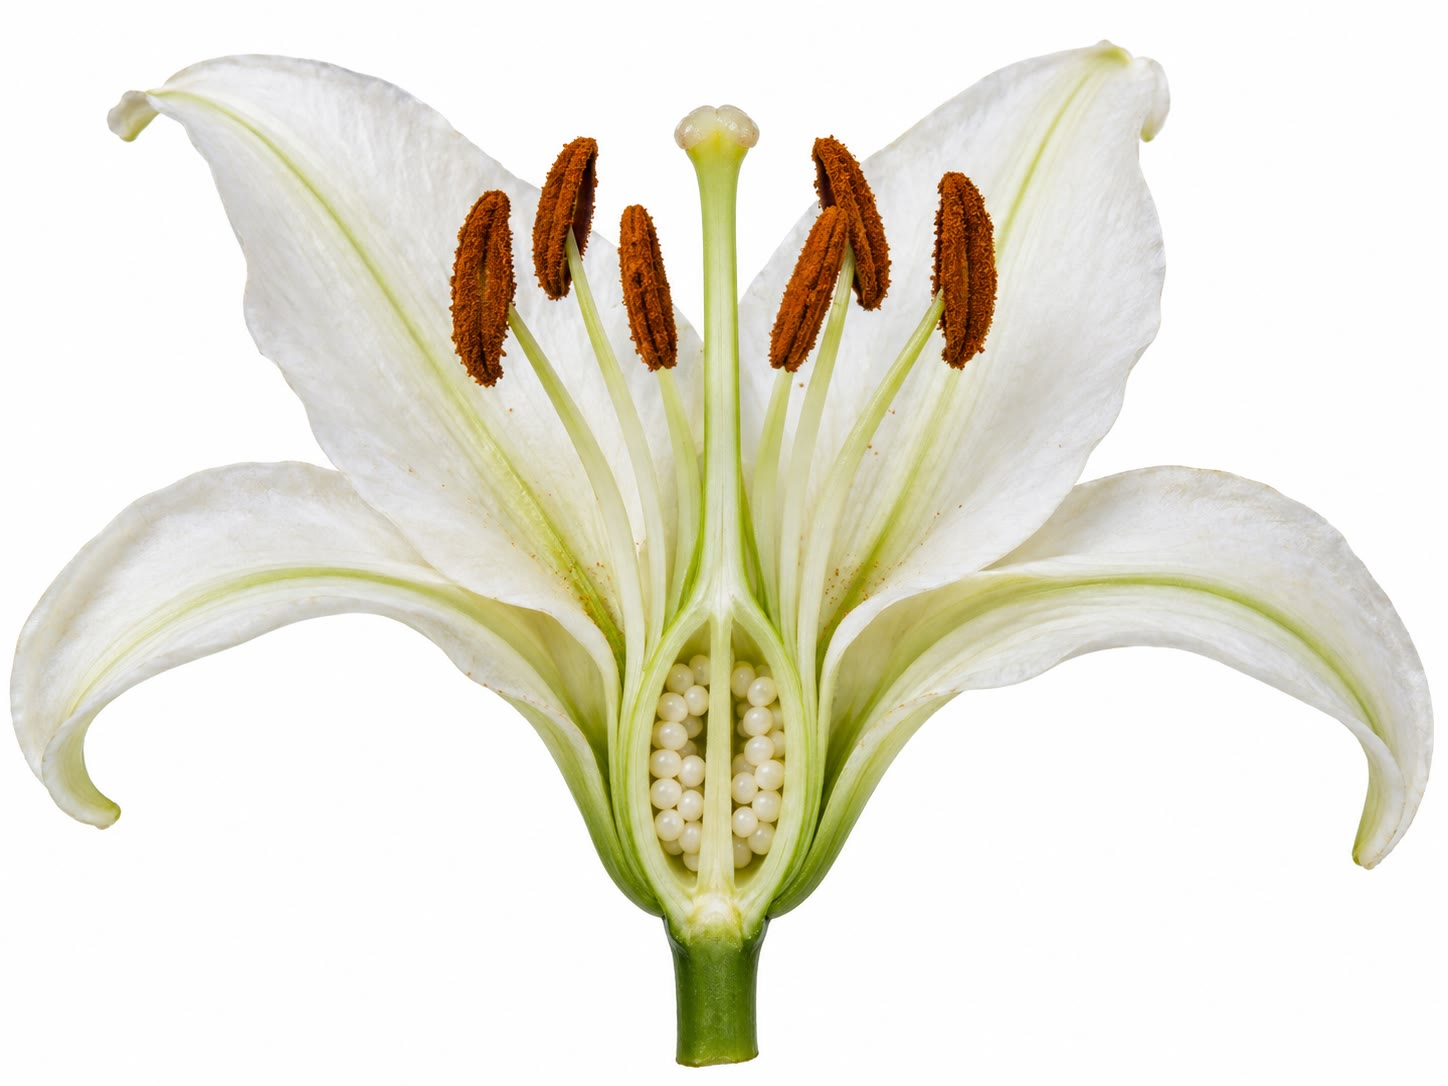
\includegraphics[width=0.55\linewidth]{images/book4/ai/b4-06-lily-dissected.jpg}

{\small लंबाई में काटी गई एक लिली: \omterm{def:b2:plant-life-cycles:heterospory}{पराग} से लदे परागकोशों वाले छह
\omterm{def:b2:angiosperm-reproduction:flower}{पुंकेसर}, चिपचिपे \omterm{def:b2:angiosperm-reproduction:flower}{वर्तिकाग्र} सहित लंबी वर्तिका, और \omterm{def:b2:plant-life-cycles:heterospory}{बीजांडों} की
पंक्तियाँ दिखाने को खोला गया \omterm{def:b2:angiosperm-reproduction:flower}{अंडाशय}।}
\end{omfigure}

\section{दोनों युग्मकोद्भिद}

\begin{proposition}[पराग: नर युग्मकोद्भिद]\label{prop:b2:angiosperm-reproduction:pollen}
\index{पराग कण}\index{लघुबीजाणुजनन}\index{स्पोरोपॉलेनिन}
हर पराग-थैली में \omterm{def:b2:meiosis-heredity:meiosis}{द्विगुणित} मातृ कोशिकाएँ \omterm{def:b2:meiosis-heredity:meiosis}{अर्धसूत्री विभाजन} से
\emph{\omterm{def:b2:plant-life-cycles:heterospory}{लघुबीजाणुओं}} के चतुष्क देती हैं। हर \omterm{def:b2:plant-life-cycles:heterospory}{लघुबीजाणु} एक बार,
असमान रूप से, विभाजित होकर एक बड़ी \emph{कायिक कोशिका} और उसी के भीतर
बंद एक छोटी \emph{जननिक कोशिका} बनाता है; और वह जननिक कोशिका, \omterm{def:b2:angiosperm-reproduction:pollination}{परागण} से
पहले या बाद में, एक बार और विभाजित होकर दो
\emph{शुक्राणु कोशिकाएँ} बनाती है। इस तरह परिपक्व \emph{\omterm{prop:b2:angiosperm-reproduction:pollen}{पराग कण}}
\qtyrange{10}{100}{\micro m} का तीन-कोशिकी \omterm{def:b2:meiosis-heredity:meiosis}{अगुणित} जीव है --- यानी पूरा नर
\omterm{def:b2:plant-life-cycles:cycles}{युग्मकोद्भिद} --- जो ऐसी भित्ति में बंद है जिसकी बाहरी परत
\emph{स्पोरोपॉलेनिन} की है, यानी ज्ञात सबसे प्रतिरोधी जैविक बहुलक की,
और जो जाति-विशेष के काँटों, छिद्रों और खाँचों से तराशी होती है, और
इसीलिए \omterm{def:b2:plant-life-cycles:heterospory}{पराग} करोड़ों वर्ष पुराने अवसादों में पौधों की पहचान करा देता
है। वह कण निर्जलित अवस्था में झड़ता है और किसी \omterm{def:b2:angiosperm-reproduction:flower}{वर्तिकाग्र} तक पहुँचने तक
घंटों (घास) से सप्ताहों (कुछ वृक्ष) तक जीता है।
\end{proposition}

\begin{omfigure}
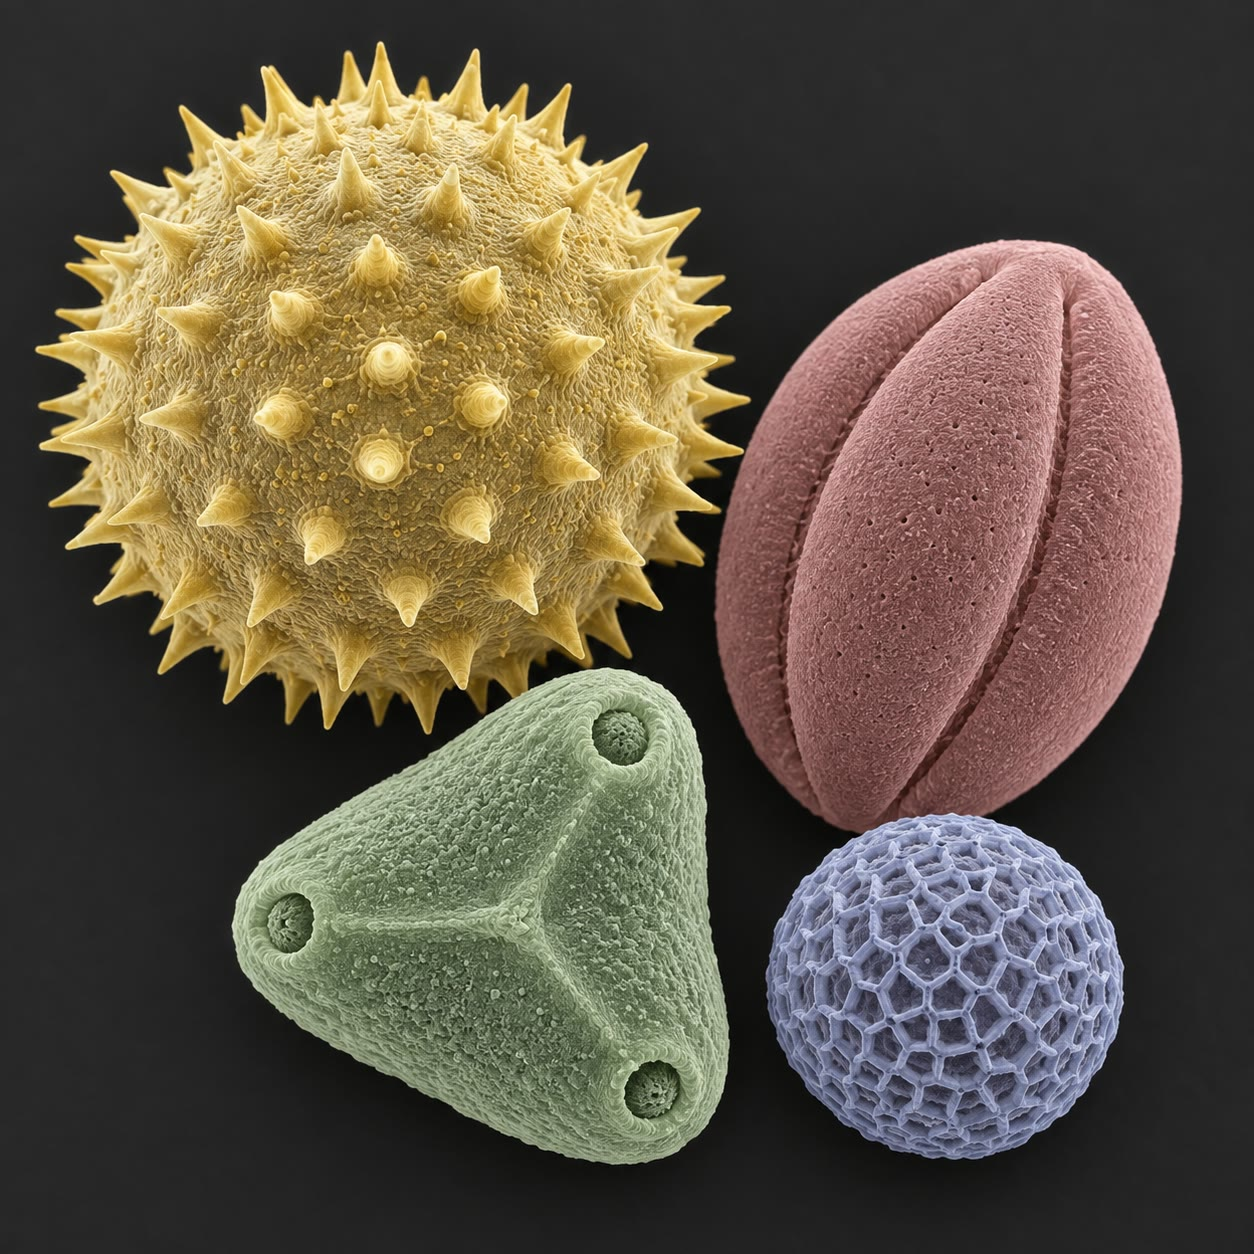
\includegraphics[width=0.45\linewidth]{images/book4/ai/b4-06-pollen-sem.jpg}

{\small क्रमवीक्षी इलेक्ट्रॉन सूक्ष्मदर्शी के नीचे \omterm{prop:b2:angiosperm-reproduction:pollen}{पराग कण}: हर जाति की
स्पोरोपॉलेनिन भित्ति की अपनी तराश है --- काँटे, खाँचे, छिद्र, एक जाल
--- जिससे उसे पहचाना जा सकता है।}
\end{omfigure}

\begin{proposition}[भ्रूणकोष: मादा युग्मकोद्भिद]\label{prop:b2:angiosperm-reproduction:embryosac}
\index{भ्रूणकोष}\index{गुरुबीजाणुजनन}\index{ध्रुवीय केंद्रक}
हर \omterm{def:b2:plant-life-cycles:heterospory}{बीजांड} में बीजांडकाय की एक \omterm{def:b2:meiosis-heredity:meiosis}{द्विगुणित} कोशिका \omterm{def:b2:meiosis-heredity:meiosis}{अर्धसूत्री विभाजन} से
गुज़रती है; चारों \omterm{def:b2:plant-life-cycles:heterospory}{गुरुबीजाणुओं} में से तीन क्षीण हो जाते हैं और चौथा,
बिना कोशिका-विभाजन के तीन समसूत्री विभाजनों द्वारा, आठ-केंद्रकी
सात-कोशिकी \emph{भ्रूणकोष} में बढ़ जाता है: बीजांडद्वारी सिरे पर
\emph{अंडाणु}, जिसके दोनों ओर दो \emph{सहायक कोशिकाएँ}; दूर के सिरे पर
तीन \emph{प्रतिमुखी} कोशिकाएँ; और बीच में एक बड़ी \emph{केंद्रीय कोशिका}
जिसमें दो \emph{\omterm{prop:b2:angiosperm-reproduction:embryosac}{ध्रुवीय केंद्रक}} हैं। बीजांडकाय में और
बीजांडद्वार वाले दो अध्यावरणों में लिपटा यह कोष ही पूरा मादा
\omterm{def:b2:plant-life-cycles:cycles}{युग्मकोद्भिद} है --- सात कोशिकाएँ, जहाँ किसी \omterm{def:b2:plant-life-cycles:moss}{मॉस} के पास एक पौधा था। दोनों
\omterm{prop:b2:angiosperm-reproduction:embryosac}{ध्रुवीय केंद्रक} अंडाणु से आनुवंशिक रूप से समरूप हैं, और यह तथ्य
भ्रूणपोष के लिए मायने रखता है।
\end{proposition}

\begin{omfigure}
\begin{tikzpicture}[every node/.style={font=\scriptsize}]
  % pollen grain
  \begin{scope}
    \draw[very thick, omProp!80!black, fill=omProp!15] (0,0) circle (1.1);
    \draw[thick, omProp!80!black] (0,0) circle (0.95);
    \foreach \a in {0,30,...,330} \draw[omProp!80!black, thick] (\a:1.1) -- (\a:1.25);
    \draw[thick, fill=omDef!25] (0.15,-0.2) ellipse (0.55 and 0.4); \node[font=\tiny] at (0.15,-0.2) {कायिक};
    \draw[thick, fill=omThm!30] (-0.3,0.45) ellipse (0.22 and 0.14); \draw[thick, fill=omThm!30] (0.2,0.5) ellipse (0.22 and 0.14);
    \draw[omThm] (0.0,0.62) -- (0.0,1.5); \node[omThm, anchor=south] at (0.0,1.5) {दो शुक्राणु कोशिकाएँ};
    \node[below, align=center] at (0,-1.4) {पराग कण ($n$)\\3 कोशिकाएँ, स्पोरोपॉलेनिन भित्ति};
  \end{scope}
  % ovule with embryo sac
  \begin{scope}[xshift=5.5cm]
    \draw[thick, fill=omExo!25] (0,0) ellipse (1.5 and 2.1);
    \draw[thick, fill=omExo!10] (0,0) ellipse (1.15 and 1.75);
    \fill[white] (-0.3,1.7) rectangle (0.3,2.2); \draw[thick] (-0.3,1.7) -- (-0.3,2.15); \draw[thick] (0.3,1.7) -- (0.3,2.15);
    \draw[thick, fill=white] (0,0) ellipse (0.7 and 1.35);
    % cells: egg + synergids top, central, antipodals bottom
    \draw[thick, fill=omThm!30] (0,0.95) circle (0.17); \node[omThm, anchor=west] at (1.6,1.2) {अंडाणु};
    \draw[thick, fill=omDef!25] (-0.35,1.0) circle (0.14); \draw[thick, fill=omDef!25] (0.35,1.0) circle (0.14); \node[anchor=west] at (1.6,0.75) {दो सहायक कोशिकाएँ};
    \draw[thick, fill=omDef!10] (0,0) ellipse (0.55 and 0.6); \fill[omDef!80!black] (-0.15,0.05) circle (0.09); \fill[omDef!80!black] (0.15,0.05) circle (0.09);
    \node[anchor=west, align=left] at (1.6,0.1) {केंद्रीय कोशिका, दो\\ध्रुवीय केंद्रकों सहित};
    \foreach \x in {-0.3,0,0.3} \draw[thick, fill=omDef!25] (\x,-1.0) circle (0.13); \node[anchor=west] at (1.6,-1.0) {तीन प्रतिमुखी};
    \draw (0.35,2.0) -- (1.6,2.0) node[right] {बीजांडद्वार};
    \draw (1.3,-0.9) -- (1.6,-1.6) node[right] {अध्यावरण};
    \draw (0.9,-1.35) -- (1.6,-2.1) node[right] {बीजांडकाय};
    \draw (1.6,1.2) -- (0.17,0.95); \draw (1.6,0.75) -- (0.49,1.0); \draw (1.6,0.1) -- (0.55,0.05); \draw (1.6,-1.0) -- (0.43,-1.0);
    \node[below, align=center] at (0,-2.3) {भ्रूणकोष सहित बीजांड ($n$)\\7 कोशिकाएँ, 8 केंद्रक};
  \end{scope}
\end{tikzpicture}

{\small किसी सपुष्पक पौधे के दोनों \omterm{def:b2:plant-life-cycles:cycles}{युग्मकोद्भिद}, और दोनों घटकर कुछ ही
कोशिकाएँ रह गए: तीन-कोशिकी \omterm{prop:b2:angiosperm-reproduction:pollen}{पराग कण}, और \omterm{def:b2:plant-life-cycles:heterospory}{बीजांड} के भीतर
सात-कोशिकी भ्रूणकोष।}
\end{omfigure}

\section{परागण}

\begin{definition}[परागण और उसके वाहक]\label{def:b2:angiosperm-reproduction:pollination}
\index{परागण}\index{परागण संलक्षण}\index{मकरंद}
\emph{परागण} किसी परागकोश से किसी \omterm{def:b2:angiosperm-reproduction:flower}{वर्तिकाग्र} तक \omterm{def:b2:plant-life-cycles:heterospory}{पराग} का हस्तांतरण है;
एक ही \omterm{def:b2:angiosperm-reproduction:flower}{पुष्प} या पौधे के भीतर \emph{स्वपरागण}, और पौधों के बीच
\emph{परपरागण}। \emph{वायु-परागित}
\omterm{def:b2:angiosperm-reproduction:flower}{पुष्प} (घास, बलूत, भोजपत्र, बरतंग) छोटे, हरे,
गंधहीन होते हैं, जिनके \omterm{def:b2:angiosperm-reproduction:flower}{वर्तिकाग्र} बड़े और पंखनुमा होते हैं और जिनका
चिकना, सूखा \omterm{def:b2:plant-life-cycles:heterospory}{पराग} विपुल मात्रा में होता है; उनका पराग-बीजांड अनुपात दस
लाख तक जाता है। \emph{प्राणी-परागित} \omterm{def:b2:angiosperm-reproduction:flower}{पुष्प} अपने वाहक को दाम चुकाते हैं:
\emph{मकरंद} (मकरंदियों से निकला शर्करा-विलयन), \omterm{def:b2:plant-life-cycles:heterospory}{पराग} स्वयं, तेल, गंध;
और वे रंग, आकार तथा गंध से विज्ञापन करते हैं, जो वाहक की
इंद्रियों के अनुरूप ढले होते हैं --- मधुमक्खियों के लिए पराबैंगनी
मकरंद-संकेत, जो पराबैंगनी देखती हैं और लाल नहीं; हमिंगबर्ड के लिए
गंधहीन लाल नलिकाकार \omterm{def:b2:angiosperm-reproduction:flower}{पुष्प};
शलभों के लिए सफ़ेद, तीव्र गंध वाले, रात में खिलने वाले गहरी नली वाले
\omterm{def:b2:angiosperm-reproduction:flower}{पुष्प}; मुर्दाख़ोर मक्खियों के लिए भूरे, दुर्गंधयुक्त \omterm{def:b2:angiosperm-reproduction:flower}{पुष्प}; चमगादड़ों
के लिए मज़बूत, हलके रंग के, रात्रि \omterm{def:b2:angiosperm-reproduction:flower}{पुष्प}। ऐसा हर लक्षण-समुच्चय एक
\emph{परागण संलक्षण} है, और \omterm{def:b2:angiosperm-reproduction:flower}{पुष्प} तथा परागक के बीच का मेल
\emph{सहविकास} का पाठ्यपुस्तकीय उदाहरण है: डार्विन ने किसी मैडागास्कर
ऑर्किड की \qty{30}{cm} मकरंद-कील से \qty{30}{cm} जीभ वाले किसी शलभ की
भविष्यवाणी की थी, जो चालीस वर्ष बाद मिला।
\end{definition}

\begin{omfigure}
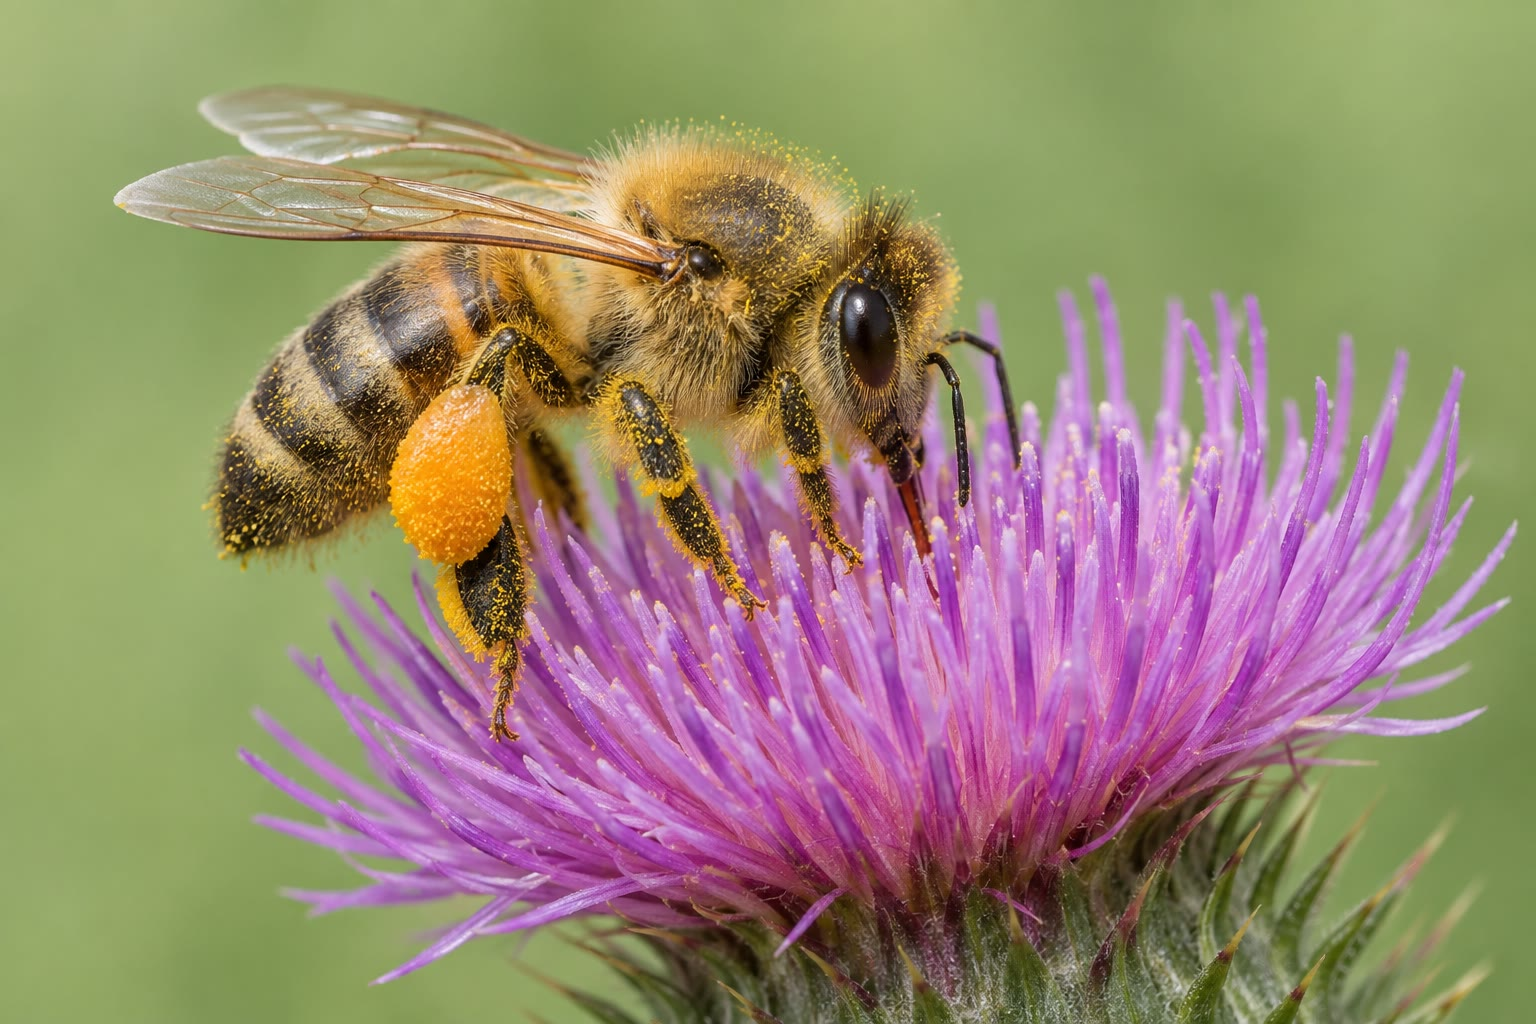
\includegraphics[width=0.58\linewidth]{images/book4/ai/b4-06-bee-on-flower.jpg}

{\small किसी ऊँटकटारे पर एक मधुमक्खी: \omterm{def:b2:plant-life-cycles:heterospory}{पराग} उसके शरीर पर छा जाता है और
उसकी पिछली टाँगों की टोकरियाँ भर देता है; उसका कुछ भाग अगले ऊँटकटारे के
\omterm{def:b2:angiosperm-reproduction:flower}{वर्तिकाग्र} तक पहुँचेगा। बैंगनी रंग, उतरने का चबूतरा और प्रचुर \omterm{def:b2:angiosperm-reproduction:pollination}{मकरंद}
मधुमक्खी-संलक्षण हैं।}
\end{omfigure}

\begin{proposition}[स्व-निषेचन से बचना]\label{prop:b2:angiosperm-reproduction:selfing}
\index{स्व-अयोग्यता}\index{विषमवर्तिकत्व}\index{भिन्नकालपक्वता}
कोई उभयलिंगी \omterm{def:b2:angiosperm-reproduction:flower}{पुष्प} स्वयं को निषेचित कर सकता है, और अनेक करते भी हैं
(मटर, गेहूँ, टमाटर); पर स्वपरागण \omterm{def:b2:meiosis-heredity:vocabulary}{अप्रभावी} हानिकारक युग्मविकल्पियों को
उजागर कर देता है (\emph{अंतःप्रजनन ह्रास}), और अधिकांश जातियाँ उसे
रोकती हैं। काल में: \emph{भिन्नकालपक्वता}, यानी परागकोश और \omterm{def:b2:angiosperm-reproduction:flower}{वर्तिकाग्र}
का भिन्न समयों पर पकना (अधिकांश छत्रकों और कंपोज़िटी में पुंपूर्वता)।
दिक् में: \emph{पृथक्केसरता}, यानी परागकोश और \omterm{def:b2:angiosperm-reproduction:flower}{वर्तिकाग्र} का अलग-अलग
रखा जाना, जैसा प्रिमरोज़ के \emph{विषमवर्तिकत्व} में, जिसके पिन \omterm{def:b2:angiosperm-reproduction:flower}{पुष्प}
(लंबी वर्तिका, नीचे परागकोश) और थ्रम \omterm{def:b2:angiosperm-reproduction:flower}{पुष्प} (छोटी वर्तिका, ऊँचे
परागकोश) \omterm{def:b2:plant-life-cycles:heterospory}{पराग} को किसी कीट के भिन्न भागों पर रखते हैं। जैवरासायनिक रूप
से: \emph{स्व-अयोग्यता}, यानी ऐसा अभिज्ञान-तंत्र जिसमें
स्त्रीकेसर से साझा कोई $S$ \omterm{def:b2:meiosis-heredity:vocabulary}{युग्मविकल्पी} ढोता \omterm{def:b2:plant-life-cycles:heterospory}{पराग} अस्वीकृत हो जाता है।
\emph{युग्मकोद्भिदी} अयोग्यता में (सेब, चेरी, पिटूनिया,
घास) \omterm{def:b2:plant-life-cycles:heterospory}{पराग} का अपना \omterm{def:b2:meiosis-heredity:meiosis}{अगुणित} $S$ \omterm{def:b2:meiosis-heredity:vocabulary}{युग्मविकल्पी} निर्णय करता है: कोई
$S_1S_2$ स्त्रीकेसर $S_1$ और $S_2$ नलिकाओं को वर्तिका में ही रोक देता
है, इसलिए किसी $S_1S_3$ पौधे का \omterm{def:b2:plant-life-cycles:heterospory}{पराग} आधा योग्य है और $S_3S_4$ का पूरा।
\emph{बीजाणुद्भिदी} अयोग्यता में (पत्तागोभी, सूरजमुखी)
\omterm{def:b2:plant-life-cycles:heterospory}{पराग} के जनक का \omterm{def:b2:meiosis-heredity:meiosis}{द्विगुणित} \omterm{def:b2:meiosis-heredity:vocabulary}{जीन-प्ररूप}, \omterm{def:b2:angiosperm-reproduction:flower}{वर्तिकाग्र} की
सतह पर, निर्णय करता है। कोई विरल $S$ \omterm{def:b2:meiosis-heredity:vocabulary}{युग्मविकल्पी} लगभग हर साथी से योग्य
होता है, इसलिए वरण किसी आबादी में दर्जनों \omterm{def:b2:meiosis-heredity:vocabulary}{युग्मविकल्पी} बनाए रखता है।
\end{proposition}
\begin{proof}[प्रमाण-सामग्री]
डार्विन (1862, 1877) ने प्रिमरोज़ का हाथ से संकरण कराया: किसी थ्रम
\omterm{def:b2:angiosperm-reproduction:flower}{पुष्प} का \omterm{def:b2:plant-life-cycles:heterospory}{पराग} किसी पिन \omterm{def:b2:angiosperm-reproduction:flower}{वर्तिकाग्र} पर (``वैध'' संगम) भरे हुए संपुट देता
था; पिन पर पिन या थ्रम पर थ्रम (``अवैध'') थोड़े ही \omterm{def:b2:angiosperm-reproduction:seed}{बीज} देता था या कोई
नहीं, जबकि पौधे स्वस्थ थे और \omterm{def:b2:plant-life-cycles:heterospory}{पराग} जीवित। उन्होंने
निष्कर्ष निकाला कि दोनों रूप परस्पर संकरण के लिए अनुकूलित हैं और
स्वपरागण से बचाए गए हैं, और हज़ारों संकरणों में प्रति संपुट \omterm{def:b2:angiosperm-reproduction:seed}{बीज}
गिनकर उन्होंने दर्जनों जातियों में स्व-निषेचन की क़ीमत नाप ली:
स्वपरागित संतति पीढ़ी-दर-पीढ़ी छोटी, हलकी और कम उर्वर थी।
\end{proof}

\begin{omfigure}
\begin{tikzpicture}[every node/.style={font=\scriptsize}]
  % pistil S1S2 with pollen tubes
  \draw[thick, fill=omDef!10] (-0.5,0) rectangle (0.5,3.2);
  \draw[thick, fill=omDef!30] (0,3.3) ellipse (0.7 and 0.2);
  \draw[thick, fill=omDef!12] (0,-0.6) ellipse (0.9 and 0.7);
  \node at (0,-0.6) {अंडाशय};
  \node[anchor=east] at (-1.1,3.3) {किसी $S_1S_2$ पौधे का वर्तिकाग्र};
  % pollen grains
  \draw[thick, fill=omThm!40] (-0.35,3.75) circle (0.13); \node[omThm, left] at (-0.5,3.75) {$S_1$};
  \draw[thick, fill=omThm!40] (0,3.75) circle (0.13); \node[omThm, anchor=south] at (0,3.92) {$S_2$};
  \draw[thick, fill=omExo!70!black] (0.35,3.75) circle (0.13); \node[right] at (0.5,3.75) {$S_3$};
  % tubes: S1 and S2 stop in the style, S3 reaches the ovary
  \draw[thick, omThm] (-0.35,3.3) -- (-0.35,2.3); \node[omThm, left, align=right] at (-0.55,2.3) {नलिका $S_1$\\रुकी हुई};
  \draw[thick, omThm] (0,3.3) -- (0,2.0);
  \draw[thick, omExo!70!black] (0.35,3.3) -- (0.35,-0.2) -- (0.2,-0.5);
  \node[right, align=left] at (0.55,0.9) {नलिका $S_3$\\किसी बीजांड तक पहुँचती है};
  \node[anchor=west, align=left, text width=6cm] at (3.2,3.2) {युग्मकोद्भिदी स्व-अयोग्यता: जिस पराग नलिका का अपना $S$ युग्मविकल्पी स्त्रीकेसर के किसी भी युग्मविकल्पी से मेल खाए वह वर्तिका में ही रोक दी जाती है};
  \node[anchor=west, align=left, text width=6cm] at (3.2,1.4) {किसी $S_1S_2$ पौधे का पराग: 0 योग्य\\$S_1S_3$ से: आधा\\$S_3S_4$ से: पूरा};
\end{tikzpicture}

{\small युग्मकोद्भिदी स्व-अयोग्यता। किसी $S_1S_2$ स्त्रीकेसर पर
$S_1$ या $S_2$ ढोती नलिकाएँ वर्तिका में रोक दी जाती हैं; कोई $S_3$
नलिका \omterm{def:b2:angiosperm-reproduction:flower}{अंडाशय} तक बढ़ जाती है।}
\end{omfigure}

\section{निषेचन}

\begin{theorem}[पराग नलिका]\label{thm:b2:angiosperm-reproduction:tube}
\index{पराग नलिका}
किसी योग्य \omterm{def:b2:angiosperm-reproduction:flower}{वर्तिकाग्र} पर कोई \omterm{prop:b2:angiosperm-reproduction:pollen}{पराग कण} फिर से जल सोखता है और एक
\emph{\omterm{thm:b2:angiosperm-reproduction:tube}{पराग नलिका}} उगाता है: कायिक कोशिका शीर्ष-वृद्धि से लंबी होती है,
शीर्ष पर \qtyrange{0.1}{1}{cm/h} की दर से नई भित्ति बिछाती है,
वर्तिका के संचारी ऊतक से होकर अपना रास्ता पचाती चलती है और उसी पर पलती
है। वह नलिका दोनों शुक्राणु कोशिकाएँ अपने शीर्ष पर ढोती है; अंतिम दूरी
में उसे सहायक कोशिकाओं के स्रावित पेप्टाइड राह दिखाते हैं, वह
बीजांडद्वार से \omterm{def:b2:plant-life-cycles:heterospory}{बीजांड} में घुसती है, किसी एक सहायक कोशिका में फूट
पड़ती है और शुक्राणु छोड़ देती है। $L$ लंबाई की किसी वर्तिका को $v$
चाल से पार करती नलिका को $L/v$ लगता है: किसी चेरी में कुछ घंटे, मक्का
में पूरा दिन, जिसके ``रेशम'' \qty{20}{cm} लंबी वर्तिकाएँ हैं। \omterm{def:b2:plant-life-cycles:heterospory}{पराग} की
जीवनक्षमता एक घड़ी बिठा देती है: घास का \omterm{def:b2:plant-life-cycles:heterospory}{पराग} घंटों में मर जाता है,
इसलिए किसी \omterm{def:b2:angiosperm-reproduction:flower}{वर्तिकाग्र} तक जल्दी पहुँचना ही होता है।
\end{theorem}
\begin{proof}
काल लंबाई बटा वृद्धि दर है; मक्का के लिए
\qty{1}{cm/h} पर \qty{20}{cm} \qty{20}{h} देता है। नलिका स्वयं
लगभग पूरी की पूरी भित्ति और शीर्ष के पीछे कोशिकाद्रव्य की एक पतली
झिल्ली भर है, इसलिए कायिक कोशिका के भंडार, और जो वह वर्तिका से सोखती है,
कण के व्यास से हज़ार गुनी लंबाई के लिए पर्याप्त हैं।
\end{proof}

\begin{proposition}[द्विनिषेचन]\label{prop:b2:angiosperm-reproduction:double}
\index{द्विनिषेचन}\index{भ्रूणपोष}
नलिका द्वारा पहुँचाई गई दोनों शुक्राणु कोशिकाओं में से एक
अंडाणु से संलयित होकर \omterm{def:b2:meiosis-heredity:meiosis}{द्विगुणित} \emph{युग्मनज} बनाती है, जिससे भ्रूण
उगता है; और दूसरी केंद्रीय कोशिका तथा उसके दोनों \omterm{prop:b2:angiosperm-reproduction:embryosac}{ध्रुवीय केंद्रकों} से
संलयित होकर एक \emph{त्रिगुणित} केंद्रक ($3n$: दो मातृ जीनोम, एक
पितृ) बनाती है, जिससे \emph{भ्रूणपोष} उगता है --- यानी ऐसा पोषक ऊतक जो
\omterm{def:b2:angiosperm-reproduction:seed}{बीज} को मंड, तेल और प्रोटीन से भर देता है। दोनों
निषेचन एक-दूसरे के मिनटों के भीतर होते हैं; और अधिकांश जातियों में
दूसरे के बिना एक भी सफल नहीं होता, इसलिए पौधा केवल उन्हीं \omterm{def:b2:angiosperm-reproduction:seed}{बीजों} को रसद
देता है जिनमें कोई भ्रूण है। भ्रूणपोष ही वह ऊतक है जो मानवता को खिलाता
है: गेहूँ और चावल का आटा, मक्का का दलिया, नारियल का सफ़ेद भाग,
सब त्रिगुणित भ्रूणपोष हैं। अनावृतबीजियों में \omterm{def:b2:angiosperm-reproduction:seed}{बीज} का भोजन-भंडार मादा
\omterm{def:b2:plant-life-cycles:cycles}{युग्मकोद्भिद} है, जो निषेचन से पहले ही बन जाता है, चाहे कोई भ्रूण बने या
न बने; जबकि आवृतबीजी का भ्रूणपोष माँग पर बनाया जाता है।
\end{proposition}
\begin{proof}[प्रमाण-सामग्री]
नवाशिन (1898) ने, किसी लिली और किसी फ्रिटिलेरी की \omterm{thm:b2:angiosperm-reproduction:tube}{पराग नलिका} का
सूक्ष्मदर्शी के नीचे भ्रूणकोष तक पीछा करते हुए, दोनों शुक्राणु-केंद्रकों
को नलिका छोड़ते देखा, और एक को अंडाणु में घुसते तथा दूसरे को
\omterm{prop:b2:angiosperm-reproduction:embryosac}{ध्रुवीय केंद्रकों} से संलयित होते; गीन्यार ने अगले ही वर्ष दूसरी
जातियों में इसकी पुष्टि कर दी। भ्रूणपोष की त्रिगुणिता गुणसूत्र-गणनाओं
से निकली, और उसके आनुवंशिक परिणाम --- किसी दाने का भ्रूणपोष
पराग-जनक के लक्षण दिखाता है (\emph{ज़ेनिया}), और वह भी दो मातृ
मात्राओं बनाम एक पितृ के अनुपात में --- मक्का के प्रजनकों ने बहुत पहले
ही देख लिए थे।
\end{proof}

\begin{omfigure}
\begin{tikzpicture}[every node/.style={font=\scriptsize}, >=stealth]
  \node[draw, rounded corners, fill=omProp!15, align=center] (sp) at (0,2) {शुक्राणु कोशिका 1 ($n$)};
  \node[draw, rounded corners, fill=omProp!15, align=center] (sp2) at (0,0) {शुक्राणु कोशिका 2 ($n$)};
  \node[draw, rounded corners, fill=omThm!15, align=center] (egg) at (4,2) {अंडाणु ($n$)};
  \node[draw, rounded corners, fill=omDef!15, align=center] (cc) at (4,0) {केंद्रीय कोशिका\\दो ध्रुवीय केंद्रक ($n + n$)};
  \node[draw, rounded corners, fill=omThm!30, align=center] (zyg) at (8.6,2) {युग्मनज ($2n$)\\$\to$ भ्रूण};
  \node[draw, rounded corners, fill=omDef!30, align=center] (endo) at (8.6,0) {भ्रूणपोष केंद्रक ($3n$)\\$\to$ भ्रूणपोष, भोजन-भंडार};
  \draw[->, thick] (sp) -- (egg); \draw[->, thick] (egg) -- (zyg);
  \draw[->, thick] (sp2) -- (cc); \draw[->, thick] (cc) -- (endo);
  \node[anchor=south] at (2,2.5) {निषेचन 1};
  \node[anchor=south] at (2,0.5) {निषेचन 2};
  \node[anchor=north, align=center] at (4.3,-0.9) {एक पराग नलिका, दो शुक्राणु कोशिकाएँ, दो संलयन: भ्रूण और उसका भोजन-भंडार साथ-साथ बनते हैं};
\end{tikzpicture}

{\small \omterm{prop:b2:angiosperm-reproduction:double}{द्विनिषेचन}: एक शुक्राणु \omterm{def:b2:meiosis-heredity:meiosis}{द्विगुणित} युग्मनज बनाता है,
दूसरा त्रिगुणित भ्रूणपोष।}
\end{omfigure}

\section{बीज और फल}

\begin{definition}[बीजांड से बीज तक, अंडाशय से फल तक]\label{def:b2:angiosperm-reproduction:seed}
\index{बीज}\index{फल}\index{बीजपत्र}\index{प्रसुप्ति}
युग्मनज विभाजित होकर एक निलंबक बनाता है, जो भ्रूण को भ्रूणपोष में
ठेलता है, और असल भ्रूण, जो गोलाकार, हृदयाकार और तर्कुरूप अवस्थाओं से
गुज़रते हुए जड़ और प्ररोह के ध्रुव तथा एक या दो \emph{बीजपत्र}
(बीज-पत्तियाँ) बिछा देता है --- यही एकबीजपत्री--द्विबीजपत्री भेद है।
अनेक द्विबीजपत्रियों में (सेम, मटर) बढ़ते बीजपत्र भ्रूणपोष सोख लेते हैं
और स्वयं ही भोजन-भंडार बन जाते हैं; और अनाजों तथा अधिकांश
एकबीजपत्रियों में भ्रूणपोष बना रहता है और इकलौता बीजपत्र एक चूषक अंग है।
अध्यावरण कड़े होकर \emph{बीज-आवरण} बन जाते हैं; बीज निर्जलित होकर
\qtyrange{5}{15}{\%} जल पर आ जाता है, उपापचय रुक जाता है, और वह
\emph{प्रसुप्ति} में चला जाता है, जो तभी टूटती है जब कोई संकेत ---
जल, ठंड, प्रकाश, आग, किसी आँत से गुज़रना --- कहे कि ऋतु ठीक है। इस बीच
\omterm{def:b2:angiosperm-reproduction:flower}{अंडाशय} की भित्ति बढ़कर \emph{फल} बन जाती है, जिसका रूप एक
प्रकीर्णन-रणनीति है: शुष्क फल जो फटते हैं (फलियाँ, संपुट) या नहीं फटते
(दाने, मेवे, पंखदार समारा), और गूदेदार फल जो खाए जाते हैं (बेरी, गुठली
वाले दृपे, सेब, जिसका गूदा पुष्पासन है); बीज उस प्राणी से बिना क्षति
गुज़र जाता है, उसका आवरण खुरच जाता है, और वह खाद के साथ कई किलोमीटर दूर
जमा कर दिया जाता है।
\end{definition}
\begin{proof}[प्रमाण-सामग्री]
अनाज का दाना दिखाता है कि अंकुरण कैसे नियंत्रित होता है। भ्रूण,
जल सोखते ही, अपने चारों ओर के भ्रूणपोष में जिबरेलिन स्रावित करता है;
भ्रूणपोष की बाहरी परत, ऐल्यूरोन, उसके उत्तर में $\alpha$-ऐमिलेज़ बनाती
और स्रावित करती है, जो मंड को उन शर्कराओं में पचा देती है जिन्हें भ्रूण
सोख लेता है। बिना भ्रूण के आधे दाने कोई ऐमिलेज़ नहीं बनाते; उनमें
जिबरेलिन डाल दीजिए तो बनाते हैं (पालेग, योमो, 1960); वह
हॉर्मोन ऐमिलेज़ जीन को चालू करके काम करता है, और यह उन पहले उदाहरणों में
से है जिनमें किसी पादप हॉर्मोन को किसी जीन तक खोजा गया। शराब बनाने वाले
इस प्रक्रिया को सहस्राब्दियों से काम में लेते आए हैं: माल्टिंग अंकुरित
कराया और फिर सुखाया गया जौ ही है।
\end{proof}

\begin{omfigure}
\begin{tikzpicture}[every node/.style={font=\scriptsize}]
  % embryogenesis stages
  \foreach \x/\lab in {0/{युग्मनज}, 1.6/{दो कोशिकाएँ}, 3.4/{गोलाकार}, 5.6/{हृदयाकार}, 8.2/{तर्कुरूप}} \node[below] at (\x,-1.1) {\lab};
  \draw[thick, fill=omThm!25] (0,-0.2) circle (0.22);
  \draw[thick, fill=omThm!25] (1.6,0.0) circle (0.2); \draw[thick, fill=omDef!15] (1.6,-0.45) circle (0.14);
  \draw[thick, fill=omThm!25] (3.4,0.1) circle (0.45); \foreach \y in {-0.5,-0.75,-1.0} \draw[thick, fill=omDef!15] (3.4,\y) circle (0.1);
  \draw[thick, fill=omThm!25] (5.6,0.0) .. controls (4.9,1.0) and (5.2,-0.6) .. (5.6,-0.6) .. controls (6.0,-0.6) and (6.3,1.0) .. (5.6,0.0);
  \draw[thick, fill=omThm!25] (5.15,0.5) circle (0.32); \draw[thick, fill=omThm!25] (6.05,0.5) circle (0.32);
  \foreach \y in {-0.75,-1.0} \draw[thick, fill=omDef!15] (5.6,\y) circle (0.09);
  \draw[thick, fill=omThm!25] (8.2,-0.2) ellipse (0.3 and 0.75);
  \draw[thick, fill=omThm!25] (7.75,0.9) .. controls (7.4,1.6) and (7.9,1.9) .. (8.05,0.55) -- cycle;
  \draw[thick, fill=omThm!25] (8.65,0.9) .. controls (9.0,1.6) and (8.5,1.9) .. (8.35,0.55) -- cycle;
  \node[omDef!80!black, anchor=west] at (9.3,-0.9) {निलंबक (नीला)};
  \node[omThm, anchor=west] at (9.3,0.9) {बीजपत्र};
  \node[anchor=west] at (9.3,-0.2) {नीचे जड़-ध्रुव};
\end{tikzpicture}

{\small किसी द्विबीजपत्री में भ्रूणजनन: युग्मनज विभाजित होकर एक भ्रूण
और एक निलंबक बनाता है; गोलाकार भ्रूण हृदयाकार हो जाता है जब दोनों
\omterm{def:b2:angiosperm-reproduction:seed}{बीजपत्र} उभरते हैं, और फिर तर्कुरूप जब जड़--प्ररोह अक्ष
लंबा होता है।}
\end{omfigure}

\begin{omfigure}
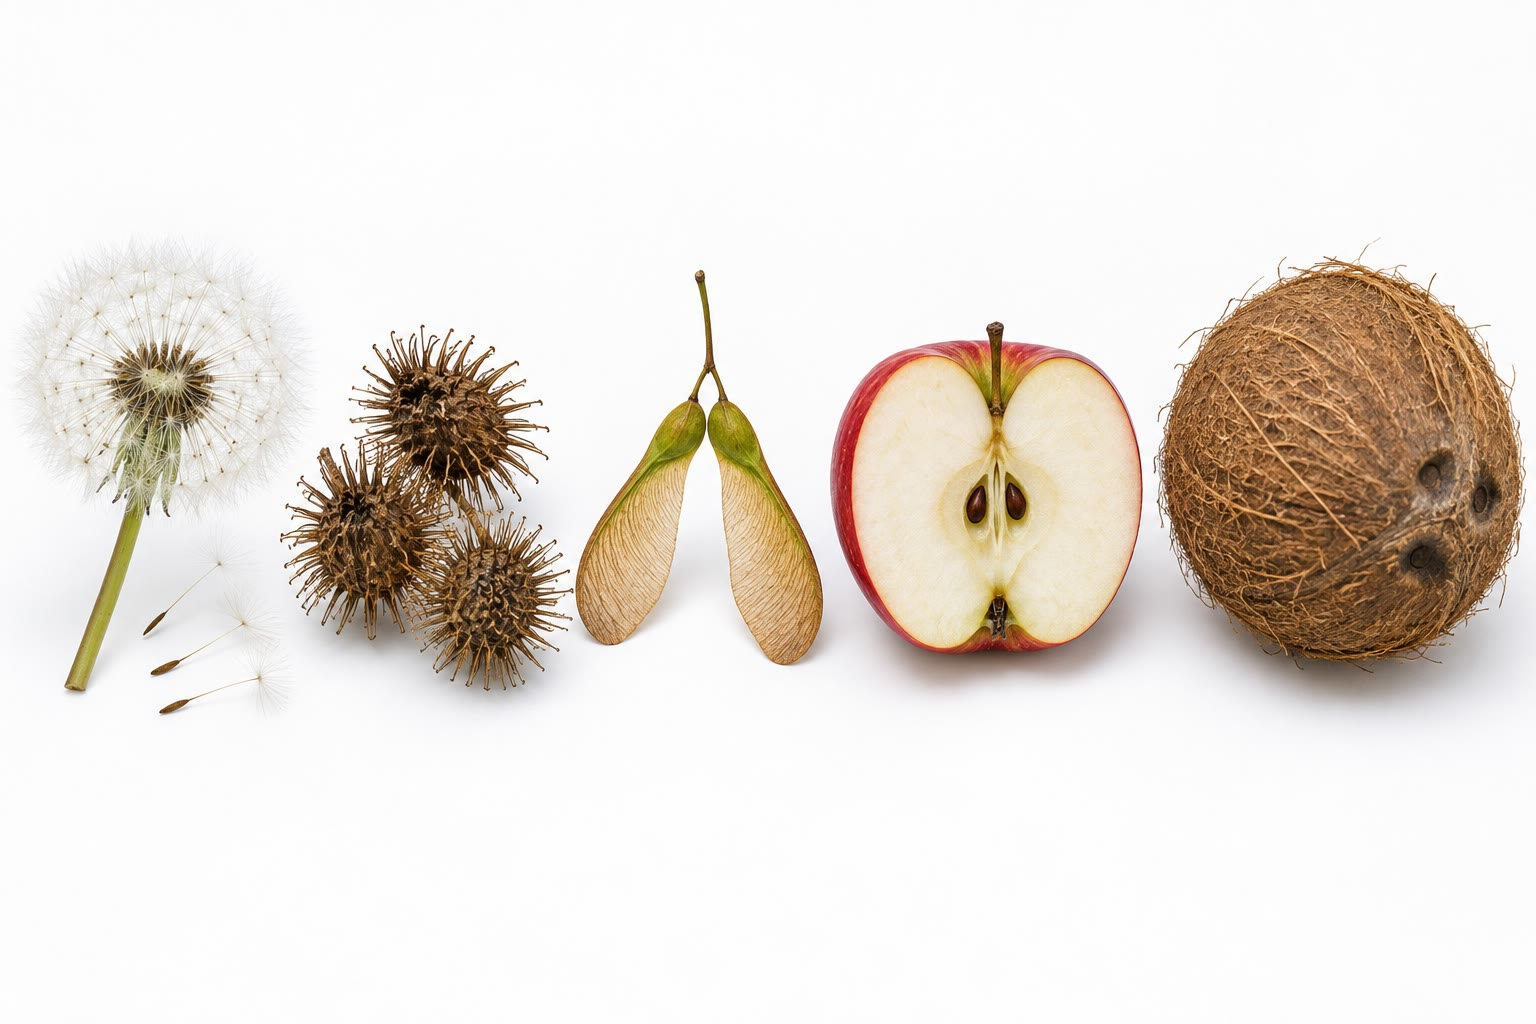
\includegraphics[width=0.62\linewidth]{images/book4/ai/b4-06-fruits-seeds.jpg}

{\small प्रकीर्णन के लिए बने \omterm{def:b2:angiosperm-reproduction:seed}{फल}: छातियाँ (डैंडेलायन), अंकुड़े
(बर्डॉक), पंख (मैपल), किसी प्राणी के लिए गूदा (सेब), और समुद्र के लिए
उतराता छिलका (नारियल)।}
\end{omfigure}

\begin{example}[प्रकीर्णन की दूरियाँ]\label{ex:b2:angiosperm-reproduction:dispersal}
डैंडेलायन का कोई कणफल अपनी छाती सहित \qty{0.3}{m/s} से उतरता है;
\qty{0.3}{m} से \qty{3}{m/s} की वायु में वह \qty{3}{m} उड़ता है, और
किसी ऊष्मीय धारा में सैकड़ों। मैपल का कोई समारा \qty{15}{m} से
\qty{1}{m/s} पर घूमता हुआ उतरता है: \qty{45}{m}। किसी पक्षी द्वारा
\qty{10}{m/s} पर बीस मिनट की उड़ान के बाद गिराई गई चेरी की गुठली:
\qty{12}{km} तक। बलूत के \omterm{def:b2:angiosperm-reproduction:seed}{फल} उसी के पैरों में गिरते हैं, जब तक कोई
जे उन्हें न ले जाए, और वह उन्हें हज़ारों की संख्या में, एक किलोमीटर और
अधिक दूर, ले जाता है और दसवाँ भाग भूल जाता है: पिछले हिमयुग के बाद
यूरोप को फिर से बसाने वाले बलूत हर वर्ष सैकड़ों मीटर उत्तर बढ़े, यानी
किसी बलूत-फल के लुढ़कने से कहीं तेज़, और उन्हें पक्षियों ने ही बढ़ाया।
\end{example}

\section{अभ्यास}

\begin{exercise}[$\star$]\label{exo:b2:angiosperm-reproduction:1}
किसी \omterm{def:b2:angiosperm-reproduction:flower}{पुष्प} के चारों चक्रों के, तथा किसी \omterm{def:b2:angiosperm-reproduction:flower}{पुंकेसर} और किसी
\omterm{def:b2:angiosperm-reproduction:flower}{अंडप} के भागों के नाम बताइए। कौन-से भाग \omterm{def:b2:meiosis-heredity:meiosis}{द्विगुणित} \omterm{def:b2:plant-life-cycles:cycles}{बीजाणुद्भिद} हैं और
कौन-से \omterm{def:b2:meiosis-heredity:meiosis}{अगुणित} \omterm{def:b2:plant-life-cycles:cycles}{युग्मकोद्भिद}?
\end{exercise}

\begin{exercise}[$\star$]\label{exo:b2:angiosperm-reproduction:2}
इनकी गुणिता बताइए: कोई \omterm{def:b2:plant-life-cycles:heterospory}{लघुबीजाणु}, कायिक कोशिका, कोई शुक्राणु कोशिका,
अंडाणु, कोई \omterm{prop:b2:angiosperm-reproduction:embryosac}{ध्रुवीय केंद्रक}, युग्मनज, भ्रूणपोष, \omterm{def:b2:angiosperm-reproduction:seed}{बीज-आवरण},
फल-भित्ति।
\end{exercise}

\begin{exercise}[$\star$]\label{exo:b2:angiosperm-reproduction:3}
किसी वायु-परागित \omterm{def:b2:angiosperm-reproduction:flower}{पुष्प} के पाँच लक्षण और किसी
मधुमक्खी-परागित के पाँच बताइए, और हर एक के लिए एक पौधा दीजिए।
\end{exercise}

\begin{exercise}[$\star$]\label{exo:b2:angiosperm-reproduction:4}
\omterm{prop:b2:angiosperm-reproduction:double}{द्विनिषेचन} क्या है, और उन दोनों संलयनों में से हर एक से क्या
बनता है? भ्रूणपोष को ``माँग पर बनाया गया'' क्यों कहा जा सकता है?
\end{exercise}

\begin{exercise}[$\star\star$]\label{exo:b2:angiosperm-reproduction:5}
मक्का का कोई रेशम \qty{25}{cm} लंबा है और कोई \omterm{thm:b2:angiosperm-reproduction:tube}{पराग नलिका}
\qty{1.2}{cm/h} से बढ़ती है। \omterm{def:b2:angiosperm-reproduction:pollination}{परागण} के बाद निषेचन में कितना समय लगता है?
कोई मंजरी दिन 0 से दिन 7 तक \omterm{def:b2:plant-life-cycles:heterospory}{पराग} झाड़ती है और उस पौधे के रेशम
दिन 5 से दिन 12 तक निकलते हैं, हर दिन उनका आठवाँ भाग; और कोई रेशम
\omterm{def:b2:plant-life-cycles:heterospory}{पराग} तभी पकड़ता है जब \omterm{def:b2:plant-life-cycles:heterospory}{पराग} झड़ रहा हो। रेशमों का कितना अंश
परागित होता है?
\end{exercise}

\begin{exercise}[$\star\star$]\label{exo:b2:angiosperm-reproduction:6}
युग्मकोद्भिदी स्व-अयोग्यता के अंतर्गत इन संकरणों में \omterm{def:b2:plant-life-cycles:heterospory}{पराग} का कितना अंश
योग्य है: $S_1S_2\times S_1S_2$, $S_1S_2\times
S_1S_3$, $S_1S_2\times S_3S_4$ (स्त्रीकेसर पहले लिखा है)? दूसरे संकरण
की संतति के \omterm{def:b2:meiosis-heredity:vocabulary}{जीन-प्ररूप} दीजिए।
\end{exercise}

\begin{exercise}[$\star\star$]\label{exo:b2:angiosperm-reproduction:7}
$n$ समान बारंबारता वाले $S$ युग्मविकल्पियों की किसी आबादी में यादृच्छिक
\omterm{def:b2:plant-life-cycles:heterospory}{पराग} का कितना अंश किसी दिए हुए पौधे से योग्य है? समझाइए कि \omterm{def:b2:genome-diversification:mutation}{उत्परिवर्तन} से
उठा कोई नया $S$ \omterm{def:b2:meiosis-heredity:vocabulary}{युग्मविकल्पी} क्यों फैलता है, और इससे
युग्मविकल्पियों की संख्या के बारे में क्या भविष्यवाणी निकलती है।
\end{exercise}

\begin{exercise}[$\star\star$]\label{exo:b2:angiosperm-reproduction:8}
मक्का का कोई \omterm{def:b2:meiosis-heredity:vocabulary}{विषमयुग्मजी} $Yy$ पौधा (पीला भ्रूणपोष \omterm{def:b2:meiosis-heredity:vocabulary}{प्रभावी})
स्वपरागित किया जाता है। उसके दानों के भ्रूणपोष के \omterm{def:b2:meiosis-heredity:vocabulary}{जीन-प्ररूप} और उनके
अनुपात दीजिए, यह याद रखते हुए कि दोनों \omterm{prop:b2:angiosperm-reproduction:embryosac}{ध्रुवीय केंद्रक} समरूप हैं।
दानों का कितना अंश पीला है? और यदि वह पौधा किसी $yy$ पौधे से परागित हो
तो?
\end{exercise}

\begin{exercise}[$\star\star$]\label{exo:b2:angiosperm-reproduction:9}
ऐल्यूरोन प्रयोग का वर्णन कीजिए और समझाइए कि वह इनके बारे में क्या
दिखाता है: (क) भ्रूण की भूमिका, (ख) जिबरेलिन की भूमिका, (ग) ऐमिलेज़
संश्लेषण का स्थल। बिना भ्रूण का आधा दाना अनिवार्य नियंत्रण क्यों है?
\end{exercise}

\begin{exercise}[$\star\star\star$]\label{exo:b2:angiosperm-reproduction:10}
वायु और प्राणी की रणनीतियों की लागत में तुलना कीजिए: कोई वायु-परागित
पौधा प्रति \omterm{def:b2:plant-life-cycles:heterospory}{बीजांड} \qty{1}{\micro g} के $10^{6}$ कण बनाता है; कोई
प्राणी-परागित पौधा प्रति \omterm{def:b2:plant-life-cycles:heterospory}{बीजांड} \qty{1}{\micro g} के $10^{3}$ कण
बनाता है और साथ में दस \omterm{def:b2:plant-life-cycles:heterospory}{बीजांडों} वाले प्रति \omterm{def:b2:angiosperm-reproduction:flower}{पुष्प} \qty{5}{mg} मकरंद-शर्करा।
हर स्थिति में प्रति \omterm{def:b2:plant-life-cycles:heterospory}{बीजांड} जनन-लागत निकालिए
(\omterm{def:b2:plant-life-cycles:heterospory}{पराग} और शर्करा की प्रति ग्राम ऊर्जा एक जैसी लीजिए), और समझाइए कि
वायु-परागण फिर भी क्यों बना हुआ है।
\end{exercise}

\begin{exercise}[$\star\star\star$]\label{exo:b2:angiosperm-reproduction:11}
\cref{ex:b2:angiosperm-reproduction:dispersal} के आँकड़ों से समझाइए कि
कोई गूदेदार \omterm{def:b2:angiosperm-reproduction:seed}{फल} किसी वृक्ष के लिए अपनी क़ीमत के योग्य क्यों है, जबकि वह
प्राणी गूदा पचा जाता है और अधिकांश \omterm{def:b2:angiosperm-reproduction:seed}{बीज} वहाँ गिराता है जहाँ वे उग नहीं
सकते।
\end{exercise}

\begin{exercise}[$\star\star\star$]\label{exo:b2:angiosperm-reproduction:12}
``बंद \omterm{def:b2:angiosperm-reproduction:flower}{अंडप} ही वह कारण है कि सपुष्पक पौधे स्थल पर छाए हुए हैं।''
इस पर विचार कीजिए: \omterm{def:b2:plant-life-cycles:heterospory}{बीजांड} का घिरा होना क्या संभव बनाता है
(\omterm{def:b2:plant-life-cycles:heterospory}{पराग} का चुनाव, अयोग्यता, \omterm{def:b2:angiosperm-reproduction:seed}{फल}) और उसकी क़ीमत क्या है।
\end{exercise}

\section{समस्या: एक बग़ीचा और एक खेत}

\begin{problem}[{सप्तांत समस्या --- सेब के किसी बग़ीचे का परागण
स्व-अयोग्यता के इर्द-गिर्द नियोजित, और मक्का के किसी खेत का निषेचन तथा
उपज उसके बनाए पराग से निकाली हुई, और अंत बग़ीचे के फल-बंधन तथा खेत की
दाना-गणना पर}]
\label{pb:b2:angiosperm-reproduction:1}
सेब युग्मकोद्भिदी रूप से स्व-अयोग्य है। किसी बग़ीचे में तीन
क़िस्में हैं: A ($S_1S_2$), B ($S_1S_3$), C ($S_3S_4$)। किसी \omterm{def:b2:angiosperm-reproduction:flower}{पुष्प} में
दो-दो \omterm{def:b2:plant-life-cycles:heterospory}{बीजांडों} वाले पाँच \omterm{def:b2:angiosperm-reproduction:flower}{अंडप} हैं, और जो \omterm{def:b2:angiosperm-reproduction:seed}{फल} पाँच से कम
\omterm{def:b2:angiosperm-reproduction:seed}{बीज} बाँधे उसे वृक्ष गिरा देता है। मधुमक्खी की एक यात्रा किसी \omterm{def:b2:angiosperm-reproduction:flower}{वर्तिकाग्र}
पर \num{100} \omterm{prop:b2:angiosperm-reproduction:pollen}{पराग कण} जमा करती है; और हर योग्य कण के किसी अब तक अनछुए
\omterm{def:b2:plant-life-cycles:heterospory}{बीजांड} को निषेचित करने की प्रायिकता $0.1$ है। कोई वृक्ष \num{5000} \omterm{def:b2:angiosperm-reproduction:flower}{पुष्प}
ढोता है और पूरी फ़सल के लिए उसे \num{250} \omterm{def:b2:angiosperm-reproduction:seed}{फल} चाहिए। मक्का: कोई मंजरी
\num{7} दिनों में $10^{7}$ कण झाड़ती है; खेत में प्रति
वर्ग मीटर \num{8} पौधे हैं; हर पौधे पर \num{600} रेशमों की एक भुट्टी
है; कोई रेशम गिरते \omterm{def:b2:plant-life-cycles:heterospory}{पराग} के सामने \qty{1e-4}{m^2} रखता है; \omterm{def:b2:plant-life-cycles:heterospory}{पराग}
\qty{0.25}{m/s} से बैठता है; और किसी दाने में \qty{0.3}{g} भ्रूणपोष है।

\medskip
\noindent\textbf{भाग I --- योग्यता।}
\begin{enumerate}
  \item A के स्त्रीकेसर पर हर क़िस्म के \omterm{def:b2:plant-life-cycles:heterospory}{पराग} के लिए योग्य अंश
        $f$ दीजिए।
  \item B के और C के स्त्रीकेसरों के लिए वही कीजिए।
  \item B के किसी वृक्ष से आती कोई मधुमक्खी किसी A \omterm{def:b2:angiosperm-reproduction:flower}{वर्तिकाग्र} पर 100
        कण जमा करती है: कितने योग्य हैं, और कितने \omterm{def:b2:plant-life-cycles:heterospory}{बीजांडों} के
        निषेचित होने की प्रत्याशा है (संतृप्ति छोड़ दीजिए)?
  \item C से और किसी दूसरे A से आती मधुमक्खी के लिए वही कीजिए।
  \item कौन-से \omterm{def:b2:angiosperm-reproduction:seed}{फल} रखे जाते हैं? केवल A क़िस्म का बग़ीचा लगाने में क्या
        जोखिम है?
  \item A वृक्षों का कोई खंड C वृक्षों से घिरा है; A तक की आधी
        मधुमक्खी-यात्राएँ C से आती हैं। यदि हर \omterm{def:b2:angiosperm-reproduction:flower}{पुष्प} को एक यात्रा मिले,
        तो A के कितने अंश \omterm{def:b2:angiosperm-reproduction:flower}{पुष्प} \omterm{def:b2:angiosperm-reproduction:seed}{फल} बाँधते हैं, और प्रति वृक्ष कितने \omterm{def:b2:angiosperm-reproduction:seed}{फल}?
        क्या फ़सल पूरी है?
  \item बग़ीचों में ऐसा कोई क्रैब-सेब बीच में क्यों लगाया जाता है जो
        सप्ताहों फूलता है, और उसके $S$ \omterm{def:b2:meiosis-heredity:vocabulary}{युग्मविकल्पी} क्यों जाँचने पड़ते हैं?
\end{enumerate}

\medskip
\noindent\textbf{भाग II --- मक्का के खेत पर \omterm{def:b2:plant-life-cycles:heterospory}{पराग}।}
\begin{enumerate}[resume]
  \item सात दिनों के औसत पर खेत के प्रति वर्ग मीटर प्रति सेकंड छोड़ा
        जाता \omterm{def:b2:plant-life-cycles:heterospory}{पराग} निकालिए।
  \item स्थायी अवस्था में बैठते \omterm{def:b2:plant-life-cycles:heterospory}{पराग} का अभिवाह छोड़े जाने की दर के
        बराबर है। वायु में \omterm{def:b2:plant-life-cycles:heterospory}{पराग} की सांद्रता (कण प्रति घन
        मीटर) निकालिए।
  \item प्रति सेकंड एक रेशम पर उतरते कणों की संख्या, और पहले कण की
        माध्य प्रतीक्षा-अवधि निकालिए।
  \item कोई रेशम एक दिन में कितने कण पाता है? केवल पहला ही उपयोगी
        क्यों है?
  \item \qty{20}{cm} का कोई रेशम परागित होता है; नलिका
        \qty{1}{cm/h} से बढ़ती है। \omterm{def:b2:plant-life-cycles:heterospory}{बीजांड} कब निषेचित होता है?
  \item कोई सूखा रेशम-निर्गमन पाँच दिन टाल देता है जबकि मंजरी
        समय पर झाड़ती है। सात-दिन की झड़ने की अवधि लेकर आँकिए कि रेशम
        पराग-ऋतु का कितना अंश पकड़ते हैं, और उपज पर इसका परिणाम क्या है।
\end{enumerate}

\medskip
\noindent\textbf{भाग III --- \omterm{prop:b2:angiosperm-reproduction:double}{द्विनिषेचन} और दाना।}
वह खेत पीले भ्रूणपोष ($Y$, \omterm{def:b2:meiosis-heredity:vocabulary}{प्रभावी}) वाली किसी क़िस्म का है और किसी
सफ़ेद ($yy$) खेत के बग़ल में है; वायु सफ़ेद खेत से बहती है।
\begin{enumerate}[resume]
  \item किसी $YY$ पौधे के उस दाने के भ्रूण और भ्रूणपोष के \omterm{def:b2:meiosis-heredity:vocabulary}{जीन-प्ररूप}
        दीजिए जो $yy$ \omterm{def:b2:plant-life-cycles:heterospory}{पराग} से निषेचित हुआ है।
  \item वह दाना पीला है या सफ़ेद? ज़ेनिया पद समझाइए।
  \item किसी $Yy$ पौधे को $yy$ \omterm{def:b2:plant-life-cycles:heterospory}{पराग} से परागित किया जाता है: भ्रूणपोष
        के \omterm{def:b2:meiosis-heredity:vocabulary}{जीन-प्ररूप} और उनकी बारंबारताएँ दीजिए।
  \item भ्रूणपोष में दो मातृ और एक पितृ जीनोम हैं।
        मात्रा-प्रभाव वाला कोई जीन प्रति प्रति 10~इकाई रंजक देता है:
        दाने $YYy$, $Yyy$ और $yyY$ (काल्पनिक रूप से दो पितृ मात्राएँ)
        कितना रंजक ढोते हैं? इनमें से कौन-सा वास्तव में हो सकता है?
  \item समझाइए कि हम भ्रूण नहीं बल्कि भ्रूणपोष क्यों खाते हैं, और यदि
        भ्रूण का भार \qty{0.03}{g} हो तो वह दाने के द्रव्यमान का कितना
        अंश है।
  \item भ्रूणपोष की ``माँग पर'' रसद अनावृतबीजी की रसद पर लाभ
        क्यों है?
\end{enumerate}

\medskip
\noindent\textbf{भाग IV --- उपज।}
\begin{enumerate}[resume]
  \item यदि \qty{90}{\%} रेशम निषेचित हों, तो प्रति भुट्टी, प्रति
        पौधा और प्रति वर्ग मीटर दाने, तथा प्रति वर्ग मीटर भ्रूणपोष
        का द्रव्यमान निकालिए।
  \item उसे टन प्रति हेक्टेयर में बदलिए।
  \item वह फ़सल प्रति वर्ग मीटर प्रति ऋतु \qty{1.2}{kg} कार्बन स्थिर
        करती है, जिसका आधा काटे गए दाने में जाता है। प्रश्न 20 के
        द्रव्यमान से संगति जाँचिए (भ्रूणपोष \qty{45}{\%} कार्बन है)।
  \item उस खेत ने प्रति काटे गए दाने कितने \omterm{prop:b2:angiosperm-reproduction:pollen}{पराग कण} झाड़े?
  \item समझाइए कि किसी बग़ीचे में अकेला मक्का का पौधा बुरी तरह भरी
        भुट्टी क्यों देता है।
  \item परिणाम बताइए: A खंड का फल-बंधन और खेत की उपज,
        दाने प्रति वर्ग मीटर तथा टन प्रति हेक्टेयर में।
\end{enumerate}
\end{problem}
